\begin{frame}{Photoplethysmography (PPG)}
    \begin{columns}
        \column{0.5\columnwidth}
        \begin{itemize}
            \item Light-based method
            \item Measures the volume of blood
            \item Similar signal to ABP
        \end{itemize}

        \column{0.5\columnwidth}
        \begin{figure}
            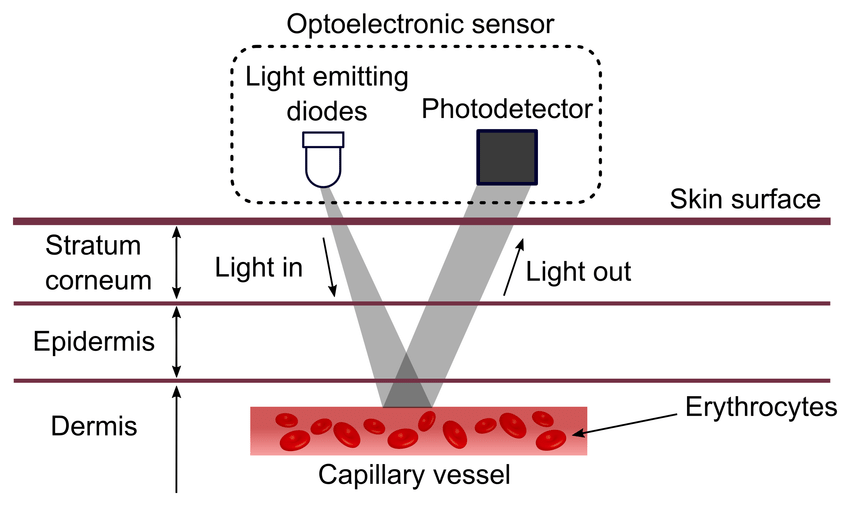
\includegraphics[width=0.6\columnwidth]{literature/ppgdiagram.png}
            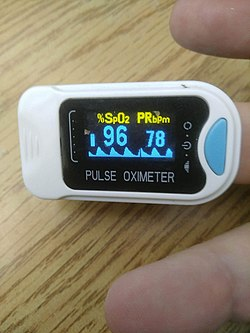
\includegraphics[width=0.3\columnwidth]{literature/ppgfinger.png}
        \end{figure}
    \end{columns}
    \begin{figure}
        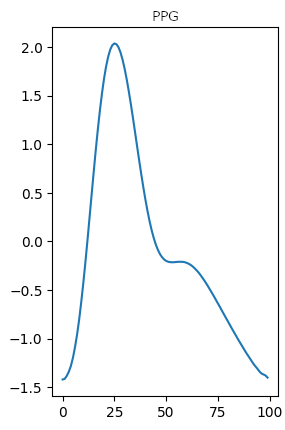
\includegraphics[width=0.25\columnwidth]{literature/signalppg.png}
        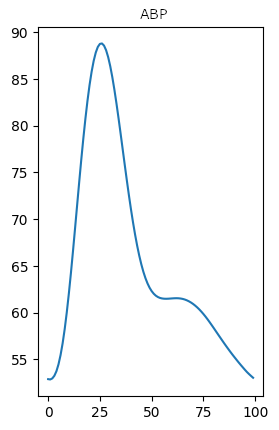
\includegraphics[width=0.25\columnwidth]{literature/singalabp.png}
    \end{figure}

\end{frame}

\begin{frame}{ML \& DL approaches}
    \begin{itemize}
        \item PPG $\to$ ABP
        \item Regression task
        \item Association for the Advancement of Medical Instrumentation (AAMI): $5\pm8$ mmHg ($MAE \pm SD$)
    \end{itemize}
    \begin{figure}
        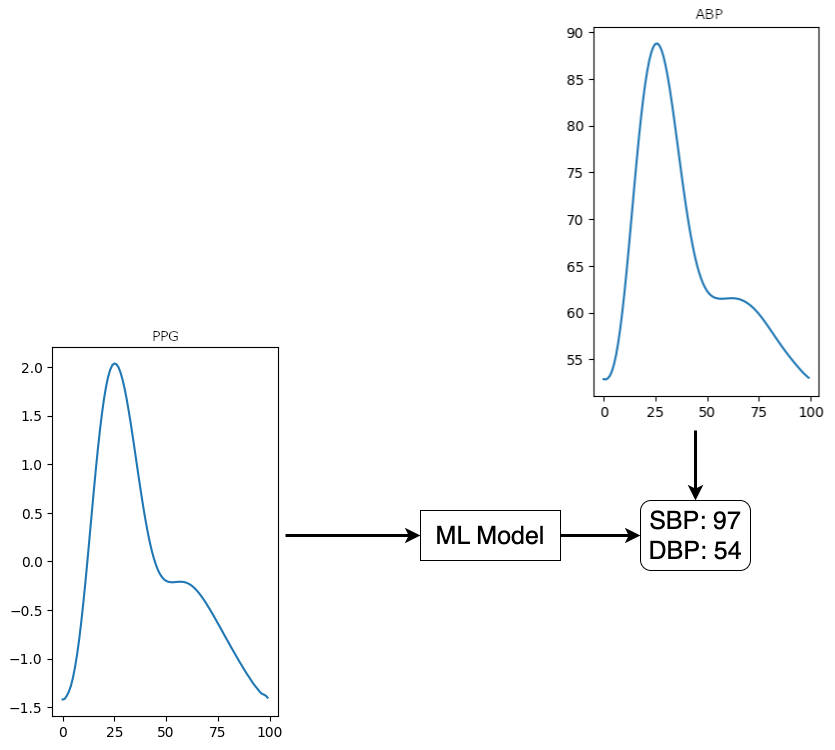
\includegraphics[width=0.5\columnwidth]{literature/regression.png}
    \end{figure}
\end{frame}

\begin{frame}{Dataset split}
    \begin{itemize}
        \item Dataset split is ambiguous
        \item Random split $\to$ data leakage
        \item Learn the physiology of a patient
        \item Patient-wise split is required
        \item Personalization is not applicable
    \end{itemize}
    \begin{figure}
        \centering
        Random split \medskip \par
        \includesvg[width=0.7\columnwidth]{literature/randomsplit.svg}

        \medskip

        Patient-wise split \medskip \par
        \includesvg[width=0.7\columnwidth]{literature/patientwisesplit.svg}
    \end{figure}
\end{frame}

\begin{frame}{Calibration-free}
    New property of the desired solution
    \begin{table}
        \begin{tabular}{r c c c}
            \hline
                             & non-invasive & continuous & calibration-free \\
            \hline
            cuff-based       & \cmark       & \xmark     & \cmark           \\
            catheter         & \xmark       & \cmark     & \cmark           \\
            ML w/ pers.      & \cmark       & \cmark     & \xmark           \\
            desired solution & \cmark       & \cmark     & \cmark           \\
            \hline
        \end{tabular}
    \end{table}
\end{frame}

\begin{frame}{Literature Gaps}
    Difficulty in comparing articles
    \begin{itemize}
        \item Dataset is not shared
        \item Preprocessing cannot be reproduced
        \item Model implementations are not published
        \item Inconsistent performance metrics
    \end{itemize}
\end{frame}